\documentclass[12pt,table,xcolor={dvipsnames}]{beamer}
\usetheme{Pittsburgh}
\usecolortheme{seagull}
%\usepackage[utf8]{inputenc}
\usepackage{fontspec}
\usepackage{amsmath}
\usepackage{listings}
\usepackage{multirow}
\usepackage{amsfonts}
\usepackage{amssymb}
\usepackage{graphicx}
\author{Design and Verification of Security Protocols and Security Ceremonies}
\title{\vspace{-.2cm}Protocol Verification Techniques - Theorem Provers}
%\setbeamercovered{transparent} 
\setbeamertemplate{navigation symbols}{} 
%\logo{
\includegraphics[scale=0.015]{Brasao_UFSC.png}
\includegraphics[scale=0.2]{brasao_PPGCC.jpg}} 
\institute{Programa de Pós-Graduacão em Ciências da Computacão \\ Dr. Jean Everson Martina} 
\date{\vspace{-1cm}August-November 2016} 
\subject{} 
\usebackgroundtemplate{
\includegraphics[width=\paperwidth,
height=\paperheight]{../reusable_images/fundo_UFSC.png}}
\begin{document}

{
\usebackgroundtemplate{
\includegraphics[width=\paperwidth,
height=\paperheight]{../reusable_images/fundo_capa.png}}
\begin{frame}
\titlepage

\includegraphics[scale=0.3]{../reusable_images/brasao_PPGCC.jpg}
\end{frame}
}

\frame{
	\frametitle{Attention!}
\begin{block}{Attention!}
This topic will be divided into two lectures. One will deal with automatic theorem provers using FOL and the second will deal with theorem provers using HOL
\end{block}
}

\frame{
\frametitle{Higher-Order Logic}
\begin{itemize}
\item Higher-order logic is a form of predicate logic that is distinguished from first-order logic by additional quantifiers and stronger semantics; \pause
\item Higher-order logics semantics are more expressive, but their model-theoretic properties are less well-behaved than those of first-order logic;\pause
\item The term "higher-order logic", abbreviated as HOL;\pause
\item HOL is any predicate logic that has greater order than Second-Order Logic;
\end{itemize}
}

\frame{
\frametitle{Higher-Order Logic}
\begin{itemize}
\item Second-Order Logic stands for the possibility of quantifying over sets;\pause
\item The idea is that you can put a quantifier over other quantifier;\pause
\item For example we can say $\forall x \exists P(x,y) \rightarrow y$\pause
\item Third-Order Logic allows for quantification over Second-Order Logic;\pause
\item Higher-order logic is the union of first-, second-, third-, …, nth-order logic;\pause
\item Higher-order logic admits quantification over sets that are nested arbitrarily deeply.
\end{itemize}
}

\frame{
\frametitle{HOL Example}
\begin{itemize}
\item First-order logic quantifies only variables that range over individuals; \pause
\item Second-order logic, in addition, quantifies over sets; \pause
\item Third-order logic also quantifies over sets of sets, and so on;\pause
\item From Second-Order Logic on we are allowed to describe mathematical induction;\pause
\item $\forall P((0\in P\land \forall i(i\in P\to i+1\in P))\to \forall n(n\in P))$\pause
\item This is the definition of the set of Natural Numbers.
\end{itemize}
}

\frame{
\frametitle{Lawrence Charles Paulson - Larry}
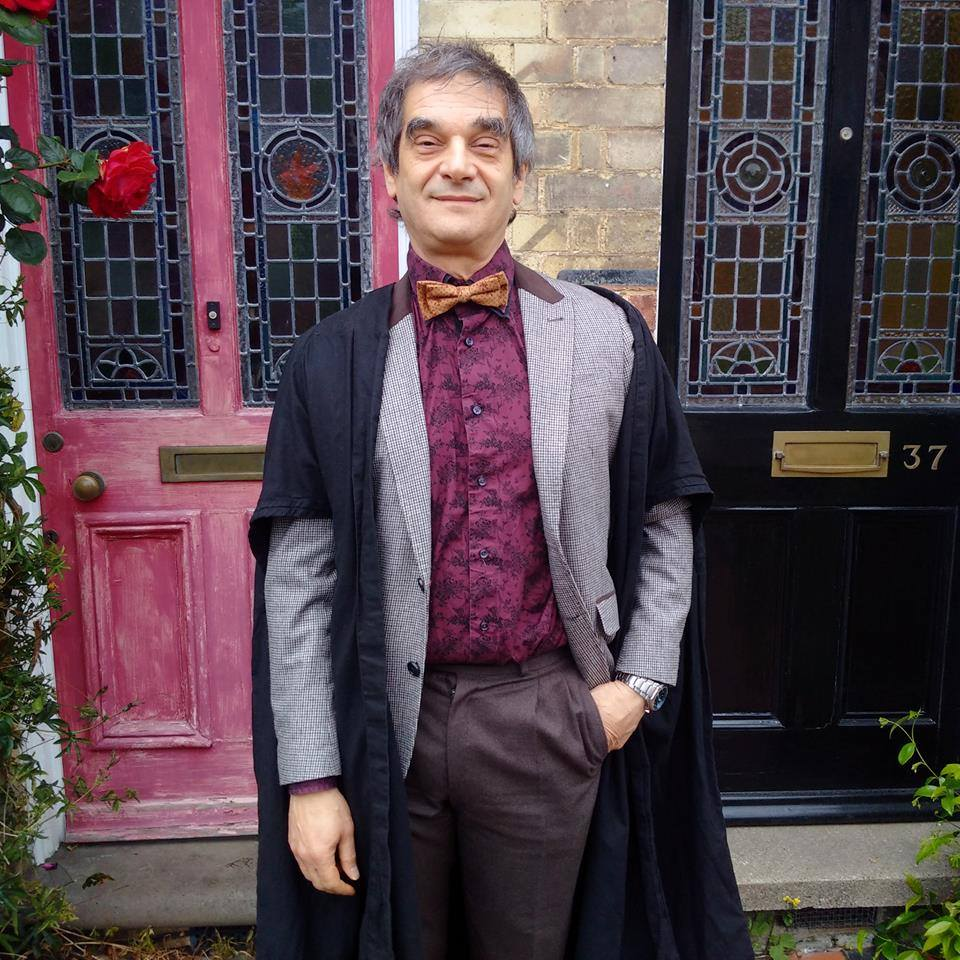
\includegraphics[scale=0.1]{larry.jpg}
\begin{itemize}
\item Lawrence Charles Paulson (Larry) is a professor at the University of Cambridge;\pause
\item His research is based around the interactive theorem prover Isabelle, which he introduced in 1986;\pause
\item He has worked on the verification of cryptographic protocols using inductive definitions;\pause
\item He has also formalized the constructible universe of Kurt Gödel;\pause

\end{itemize}
}

\frame{
\frametitle{Curiosities about Larry}
\begin{itemize}
\item He was one of the most cited researchers on a paper that demonstrated the existence of God by a machine on Gödel's world;\pause
\item He is a deep minded atheist;\pause
\item He has a page called: "Larry Paulson - Portrait of a God";\pause
\item http://www.geocities.ws/robrich18/Larry.html
\begin{center}

\includegraphics[scale=0.3]{LarryBond.jpg}
\end{center}
\end{itemize}
}

\frame{
\frametitle{Larry's Protocol Verification Time-line}
\begin{itemize}
\item Isabelle theorem prover;\pause
\begin{itemize}
\item General tool; \pause
\item Works with protocols since 1997;\pause
\end{itemize}
\item Many papers describing the Inductive Method he created;\pause
\item Many case studies, including:\pause
\begin{itemize}
\item Verification of SET protocol (6 papers)\pause
\item Kerberos (3 papers)\pause
\item TLS protocol\pause
\item Yahalom protocol, smart cards, etc\pause
\end{itemize}
\item Last work published in 2015: "Verifying multicast-based security protocols using the inductive method. Martina, J.E., Paulson, L.C."
\end{itemize}
}

\frame{
\frametitle{The Inductive Method}
\begin{itemize}
\item Starts with an informal protocol description;\pause
\item Out of that we extract:\pause
\begin{itemize}
\item An inductive abstract trace model;\pause
\item Correctness theorem about the traces;\pause
\end{itemize}
\item We then add the attacker inference rules;\pause
\item We stated the goals ad theorems and lemmas;\pause
\item We prove the theorems inductively to demonstrate correctness.
\end{itemize}
}


\frame{
\frametitle{The Inductive Method Mechanics}
\begin{itemize}
\item Larry Paulson advocates a simple approach: \pause
\begin{itemize}
\item A protocol in a context describes a set of traces;\pause
\item These traces are defined inductively;\pause
\item A specification is again a property of traces;\pause
\item Checking requires proving that all the traces satisfy the property, by induction on the construction of the traces;\pause
\item Main point: these proofs are big, uninteresting, and better left to machines;\pause
\item Use a theorem prover (Isabelle)to write the proofs.
\end{itemize}
\end{itemize}
}

\frame{
\frametitle{Isabelle}
\begin{itemize}
\item Automated support for proof development, which supports:\pause
\begin{itemize}
\item Higher-order logic;\pause
\item Serves as a logical framework;\pause
\item Supports ZF set theory and HOL;\pause
\item Generic treatment of inference rules;\pause
\end{itemize}
\item Powerful simplifier, classical reasoner and connected tools;\pause
\item Strong support for inductive definitions.
\end{itemize}
}

\frame{
\frametitle{Inductive Method Support in Isabelle}

Due to my lack of time we will jump to my Ph.D Thesis to get the explanation from there. I promise next time it will be everything on the slides..

}

 
\frame{
	\frametitle{Discussion}
\begin{itemize}
\item What else can you foresee modelled using this strategy?\pause
\item Can this be extended?\pause
\item What this strategy can not do?
\end{itemize}
}

{
\usebackgroundtemplate{
\includegraphics[width=\paperwidth,
height=\paperheight]{../reusable_images/fundo_capa.png}}
\begin{frame}

{\LARGE Questions????}

\end{frame}
}

{
\usebackgroundtemplate{
\includegraphics[width=\paperwidth,
height=\paperheight]{../reusable_images/fundo_capa.png}}
\begin{frame}

\includegraphics[scale=0.8]{../reusable_images/cc_logo_arge.png}\hspace{0.5cm} 

\includegraphics[scale=0.95]{../reusable_images/by.png}

\vspace{1cm}
This work is licensed under the Creative Commons Attribution 4.0 International License. To view a copy of this license, visit http://creativecommons.org/licenses/by/4.0/.
\end{frame}
}

\end{document}